%! Author = ben
%! Date = 23.10.2023

\documentclass[./entry.tex]{subfiles}
\usepackage{biblatex}
\usepackage{multirow}
\usepackage{colortbl}
\usepackage{lipsum}

\begin{document}
    \chapter{Anhang}

    \paragraph{Lineare\ Datenstrukturen}
    Lineare Datenstrukturen sind Datenstrukturen, die die Elemente in einer bestimmten Reihenfolge speichern. Die
    Reihenfolge wird durch die Reihenfolge der Elemente bestimmt. Die Elemente werden nacheinander gespeichert und
    können nur über die Position im Speicher angesprochen werden. Die bekannteste linearen Datenstrukture ist
    das Array.

    \paragraph{Big-O Notation}
    Die Big-O-Notation ist eine mathematische Notation, die verwendet wird, um das asymptotische Verhalten von
    Funktionen zu beschreiben. Sie wird in der Informatik verwendet, um die Laufzeit von Algorithmen zu beschreiben.
    Die Big-O-Notation wird verwendet, um die Laufzeit eines Algorithmus in Abhängigkeit von der Anzahl der zu
    sortierenden Elemente zu beschreiben. Dabei wird die Anzahl der zu sortierenden Elemente mit $n$ bezeichnet.
    Die Laufzeit wird in Abhängigkeit von $n$ angegeben. Die Laufzeit wird mit $O(n)$ angegeben. Dabei ist $O(n)$
    die obere Schranke der Laufzeit.
    \footnote{\bscite{big-o-notation}}

    \begin{multicols}{2}

        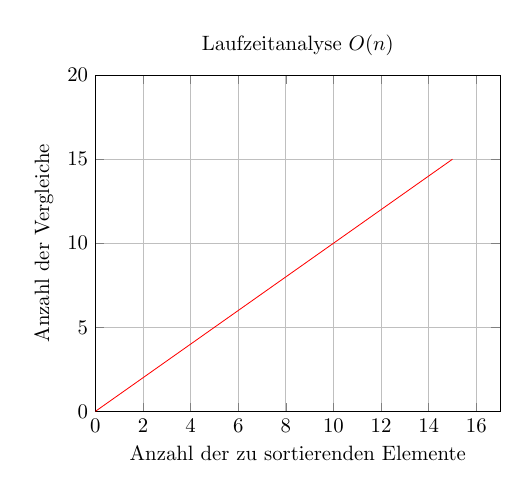
\begin{tikzpicture}[scale=0.75]
            \begin{axis}
                [
                title={Laufzeitanalyse $O(n)$},
                xlabel={Anzahl der zu sortierenden Elemente},
                ylabel={Anzahl der Vergleiche},
                grid,
                xmin=0,
                xmax=17,
                ymin=0,
                ymax=20
                ]

                \addplot[domain=0:15, color=red]{x};
            \end{axis}
        \end{tikzpicture}

        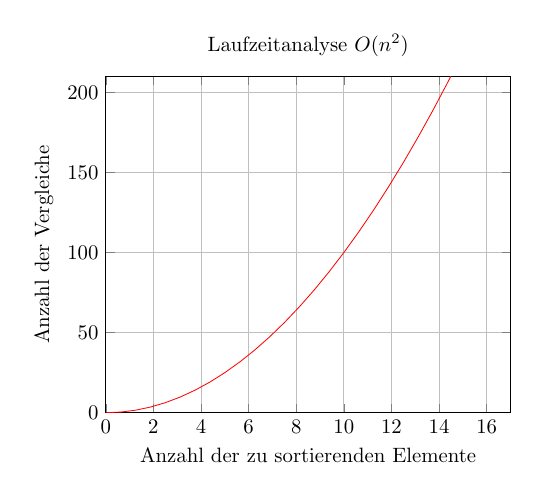
\begin{tikzpicture}[scale=0.75]
            \begin{axis}
                [
                title={Laufzeitanalyse $O(n^2)$},
                xlabel={Anzahl der zu sortierenden Elemente},
                ylabel={Anzahl der Vergleiche},
                grid,
                xmin=0,
                xmax=17,
                ymin=0,
                ymax=210
                ]

                \addplot[domain=0:15, color=red]{x^2};
            \end{axis}
        \end{tikzpicture}
    \end{multicols}

\end{document}